\documentclass[../../main.tex]{subfiles}

\usepackage{pgfplots}

\begin{document}

\chapter{Results}

A number of experiments were conducted with two broad goals: verifying that at least some of the proposed options work on simplified abstract engineering environments, and proving that the proposed architecture has desirable qualities in more complex environments.
Some experiments were also carried out to visualise and explore the latent space mappings in an intuitive way.

\section{Approach verification}

\subsection{Distribution distance}

Due to the potential issues with minimising KL-divergence discussed in \S 4.1.2, a highly simplified environment was devised in which the target distribution is known.
The target distribution was fixed as a standard normal distribution (constraints were not considered at this stage) and the generator's output distribution was modelled as a normal distribution whose mean and standard deviation were controllable parameters.

Although KL-divergence is analytically tractable for two normal distributions, it was estimated through sampling of the generated distribution as described in \S 4.1.1.
Trained variables were initialised such that the standard deviation started at $1$, while the initial mean was varied.

The mean $\mu$ and standard deviation $\sigma$ after each batch are shown in Figure \ref{fig:broadKLDivergence}.

\begin{figure}
    \begin{center}
    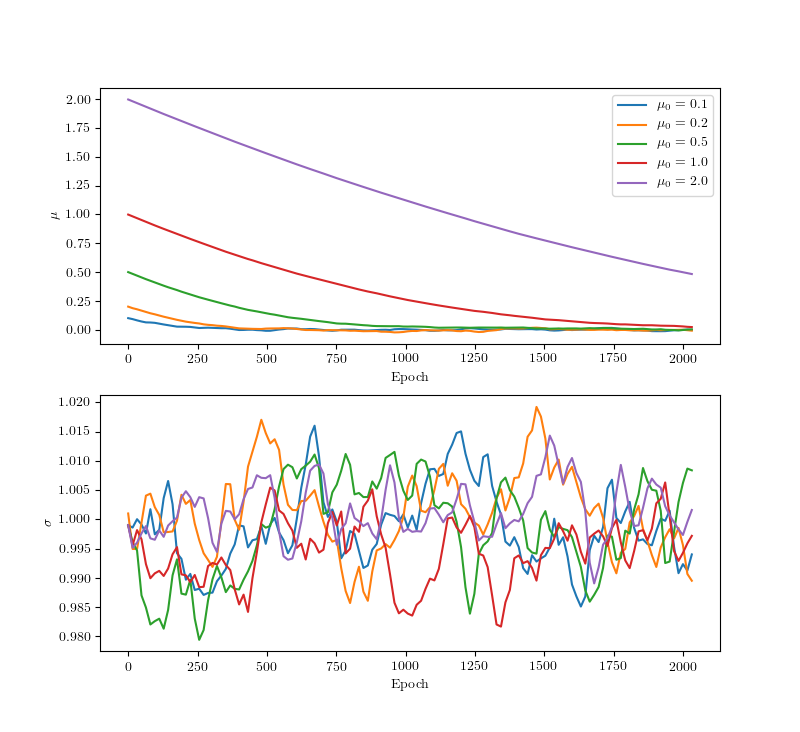
\includegraphics[scale=0.65]{broadKLDivergence.png}
    \caption{
        Change in $\mu$ and $\sigma$ over time when training arbitrary normal distributions with different starting means to match the standard normal distribution. 
        Parameters were updated using the Adam optimisation algorithm to minimise KL-divergence, as estimated by taking samples from the varying distribution in batches of 64.
    }
    \label{fig:broadKLDivergence}
    \end{center}
\end{figure}

\subsection{Precision proxy optimisation}
\subsection{Recall proxy optimisation}
\subsection{Pretraining}
\subsection{Constraint embeddings}

\section{Method properties}
\subsection{Expected satisfaction probability}
\subsection{Relative density of true solutions}
\subsection{Effect of recall weight}
\subsection{Multimodal solution sets}
\subsection{Equality constraints}

\section{Latent space properties}

\section{Application to complex problems}

\end{document}
